The vague context-dependent nature of gradable adjectives has been promisingly formalized in models within the Rational Speech Act framework -  a suite of game-theoretically oriented recursive models of pragmatic language understanding \parencite[e.g.,][]{goodman2016, lassiter2017adjectival, tessler2017warm}. Introduced by \textcite{frank2012predicting}, the Rational Speech Act framework is well in line with recent insights in the increasingly influential Bayesian cognitive modelling tradition, showing a great deal of flexibility to account for various pragmatic phenomena like scalar implicature, hyperbolic language or generics, among many others \parencite[e.g.,][]{tenenbaum2011grow, problang}. This chapter reviews the basics of Rational Speech Act models and specifically prior models of gradable adjectives, to finally propose a minimal extension of existing models formalizing the reference-predication trade-off hypothesis, allowing to flexibly incorporate reasoning about context and role of the noun in comparison class inference. 
  
\section{Understanding Rational Speech Act Models}

Language is fascinatingly flexible and efficient; this is largely due to the fact that interlocutors do not have to encode all information explicitly in utterances they produce, but instead rely on each other's ability to infer many aspects of meaning from linguistic and situational context. In particular, pragmatic models of communication posit that given these contextual constrains, speakers and listeners can efficiently \emph{reason about each other's intended meaning} under one important assumption: speakers are approximatly \emph{rational} with respect to their intended goal \parencite{frank2012predicting}. The Rational Speech Act approach (henceforth: RSA) views communication as recursive reasoning between speaker and listener: in interpretation-oriented models, a pragmatic listener $L_1$ infers a state of the world intended to be conveyed by a rational speaker, by using \emph{Bayesian inference} to reason about likely world states given the observed utterance, knowing that the rational speaker $S_1$ chooses the utterance according to its most likely semantic interpretation by a literal listener $L_0$ \parencite{problang}.  

The idea of language as rational action produced by \emph{cooperative} interlocutors was formulated by \textcite{grice1975logic}. The core of his proposal are four conversational maxims that speakers are thought to stick to when producing utterances in order to convey particular messages: the \emph{maxims of relation} (contributions made to the conversation are relevant), \emph{quantity} (the contributions are as informative as required, but not more so), \emph{quality} (the speaker believes their contributions to be true) and \emph{manner} (the way the contributions are expressed is perspicuous). Listeners then reason about intended messages in light of these maxims \parencite{grice1975logic}.

Grice’s ideas became particularly influential when precise information-theoretic formalisations of such vague concepts like \emph{informativeness, cooperation} and \emph{relevance} were proposed, and, informed by insights from game-theory, gave rise to RSA \parencite{frank2012predicting}.
In particular, RSA proposes that coordination of intended meaning between interlocutors can be captured via iterative application of probabilistic mechanisms, and context-dependence of utterance meaning can be captured as listener uncertainty about the message encoded in utterances by the speaker (i.e., the state of affairs in the world she wishes to communicate) - in Bayesian cognitive modelling spirit as \emph{subjective beliefs} of the listener - that is, as a \emph{probability distribution} over possible states of the world \parencite{tenenbaum2011grow}. The listener agent can then update her beliefs about the world upon learning a proposition via Bayes' rule - namely upon hearing an utterance $u$ produced by an informative speaker $S_1$ \parencite{frank2012predicting}.

These mechanisms of RSA are best illustrated by a simple example from a reference game, as described by \textcite{frank2012predicting}:
Consider a simple world consisting of a context $C$ = \{blue square, blue circle, green square\} (Fig. \ref{rsa-scene}).
\begin{figure*}[t]
	\begin{center}
		
\includegraphics[width=0.5\linewidth]{rsa_scene.png}
	\end{center}
	\vspace{-0.3cm}
	\caption{A simple reference resolution example scenario: the context $C$ consists of three possible referents \parencite{frank2012predicting}}
	\label{rsa-scene}
\end{figure*}
In such a reference game scenario, a speaker wants to communicate to a listener a particular referent $s$ in context $C$, e.g., the blue square. To do so, let us assume she has a finite set of utterances $U = \{blue, green, square, circle\}$.  \footnote{The finite fixed set of alternative utterances is a crucial assumption made in RSA. It is a highly relevant question for future research how human interlocutors actually determine the set of relevant alternatives.} A listener then tries to recover the intended referent (i.e., the blue square) upon receiving an utterance (e.g., "blue"). 
As briefly mentioned above, standard RSA models consist of three layers: a pragmatic speaker $S_1$ who chooses an optimal utterance for signalling $s$ (the blue square) to a literal listener $L_0$, who infers all the referents consistent with the literal meaning of the utterance $u$ ('blue'), and a pragmatic listener $L_1$ who reasons about this speaker behaviour given a particular utterance $u$ ('blue'), using Bayes' rule.

So the basis of every RSA model is the na\"ive literal listener agent $L_0$ that $S_1$ reasons about when choosing an optimal utterance to communicate the blue square, that computes a probability distribution over referents of context $C$  consistent with the received utterance $u$ (i.e., conditioning on $\llbracket u \rrbracket (s) = 1$): %\pt{function that maps each utterance to the probability distribution over world states}

$$P_{L_0}(s | u, C) = \frac{\llbracket u \rrbracket (s) \times P(s)}{\sum_{s' \in C} \llbracket u \rrbracket (s') P(s')}$$
The context $C$ is typically assumed to be shared between speaker and listener, so it will be dropped in further derivations for simplicity. Given that the denominator is a constant, it can also be dropped for simplicity, so that the probability of a particular state $s$ given $u$ is \emph{proportional} to the literal meaning of $\llbracket u \rrbracket (s)$ and the prior probability of $s$: 
$$P_{L_0}(s | u) \propto \llbracket u \rrbracket (s) \times P(s)$$
The prior $P(s)$ is the prior belief of $L_0$ about which states are likely to be communicated by the speaker. Typically, a uniform prior is used, indicating that a priori any state is as likely as others, but relevant contextual information like perceptual salience or frequency of some referents might be encoded in this prior \parencite{frank2012predicting}.
  
So for our example utterance 'blue' the literal listener $L_0$ infers the following distribution (Table \ref{rsa-l0}), since the utterance equally applies to two objects in the example context:

\begin{table}[h]
\begin{center}
	\caption{The probability distribution over states inferred by $L_0$ when hearing the utterance 'blue'}
	\label{rsa-l0}
	\vskip 0.12in
	\begin{tabular}{cc}
		State & Probability \\
		\hline
		blue circle & 0.5 \\
		blue square & 0.5 \\
		\hline
	\end{tabular}
\end{center}
\end{table}
One crucial component of the $L_0$ is the \emph{literal meaning} of the observed utterance $u$. In RSA, literal semantics computation is based on a form of Montague’s compositional semantics, classically assuming a mapping from particular states to Boolean truth-values \parencite{montague1973proper} \parencite[but see e.g.][for alternative approaches]{degen2020redundancy}. 
So, for instance for the context Fig. \ref{rsa-scene}, applying the utterance 'circle' to the blue square would return \texttt{false}, but 'blue' would be \texttt{true}:
$$\llbracket circle \rrbracket (blue \: square) = 0$$
$$\llbracket blue \rrbracket (blue\: square) = 1$$

The next RSA layer, $P_{S_1}(u | s)$, incorporates the notion of a cooperative speaker. Specifically, $S_1$ is modelled as an agent who chooses an utterance $u$ rationally, i.e., according to its expected utility in order to communicate a particular state of the world $s$ in context $C$ to $L_0$. This is captured in the speaker-utility function $U_{S_1}(u; s)$, which trades-off the informativity of an utterance for $L_0$ with non-negative cost $C(u)$ of producing the particular utterance over other available options\parencite{problang}:
$$U_{S_1} (u;s) = log L_0(s | u) - C(u)$$
In information-theoretic terms, $L_0$ provides a hook to compute the \emph{informativeness} of particular utterances as communicating particular states within this utility function, 
where informativeness is quantified by the utterance's surprisal - a measure of how much uttering a particular $u$ reduces uncertainty about the state of the world, given that $u$ is \emph{true of $s'$} (i.e., $\llbracket u \rrbracket (s') = 1$) \parencite{frank2012predicting}: 
$$I_{ \tilde{u} (s')}(s') = -log(\tilde{u} (s'))$$
$I_{\tilde{u} (s')}(s')$ measures how much information is gained when hearing the utterance $u$, assuming a known distribution $\tilde{u} (s')$ over states of the world that are coveyed by the literal interpretation $\llbracket u \rrbracket$, implying the probability of $s'$; i.e., it measures how \emph{surprising} it would be to observe $s'$ upon observing $u$.
Intuitively, assuming a uniform $\tilde{u} (s')$, the less states an utterance applies to, the lower is the surprisal of a particular state, and the higher is its informativeness. For instance, in the context of Fig. \ref{rsa-scene}, the utterance 'circle' is highly informative, because there is only one object it applies to, while the utterance 'blue' is less informative because it applies to two objects. 
Therefore, the speaker utility is anti-proportional to the surprisal of the utterance, resulting in \parencite{frank2012predicting}:
$$U_{S_1} (u;s) = -(-log(\tilde{u}(s))) - C(u) = log L_0(s| u) - C(u)$$  %: speakers strive to choose an utterance minimizing surprisal of a particular state of the world given that utterance. 
The cost function $C(u)$ is also an important hook for integrating psychologically plausible information about speaker-biases, like frequency or complexity of particular utterances comapred to others. Now the rational speaker $S_1$ maximizes the probability of conveying the intended state of the world $s$, acting according to Bayesian decision theory by choosing an utterance $u$ proportionally to its expected utility (see above) described by a \emph{softmax} function:

$$P_{S_1}(u | s) = \frac{e^{\alpha U_{S_1} (u; s)}}{\sum_{u' \in U s.t. u'(s) = true} e^{\alpha U_{S_1} (u'; s)}}$$
For this example, $S_1$ chooses an utterance $u$ maximizing the probability of the state 'blue square' being recovered by $L_0$. So, $S_1$ infers a distribution over utterance applicable to the target 'blue square' (Table \ref{rsa-s1}):

\begin{table}[h]
	\begin{center}
		\caption{The probability distribution over utterance inferred by the pragmatic speaker $S_1$ in order to communicate the referent 'blue square'}
		\label{rsa-s1}
		\vskip 0.12in
		\begin{tabular}{cc}
			Utterance & Probability \\
			\hline
			blue & 0.5 \\
			square & 0.5
		\end{tabular}
	\end{center}
\end{table}
The parameter $\alpha$ controls the speaker's \emph{optimality}, assuming $\alpha = 1$ in examples used here; for $\alpha = \infty $ the fully rational decision rule used in game-theory can be recovered \parencite{problang, lassiter2017adjectival}.
 
Finally the top-level layer, the pragmatic listener $L_1$, reasons about this utterance-generating speaker behaviour given a particular utterance $u$ ('blue'), using Bayes' rule: \footnote{This recursive depth of three model layers is a common assumption in RSA models, and requires a reasonable amount of computational resources \parencite{lassiter2017adjectival}. Yet this is just a practical approximation, and some models (e.g., production-oriented models ) employ additional levels\parencite{problang}.}
 
$$P_{L_1}(s | u) = \frac{P_{S_1}(u | s) P(s)}{\sum_{s' \in C} P_{S_1}(u | s') P(s')}$$
That is, the probability of a particular state $s$ (i.e., blue square) given the utterance $u$ ('blue') is equal to the probability that the pragmatic speaker $S_1$ would choose $blue$ in order to communicate about the \textit{blue square}, multiplied by the prior probability $P(s)$ of occurence of state $s = blue \:square$, normalised by a constant sum of probabilities of all possible speaker behaviors for all possible states $s'$. Since the denominator is a constant, it can be dropped, resulting in the probability of a particular $s$ given $u$ being \emph{proportional} to the speaker production probability $P_{S_1}(u | s)$ times the state prior $P(s)$:
$$P_{L_1}(s | u) \propto P_{S_1}(u | s) P(s)$$ 
Interestingly, the state prior $P(s)$ might differ between $L_0$ and $L_1$, e.g. incorporating prior world knowledge of the pragmatic agent $L_1$, but being uniform for the na\"ive agent $L_0$ \parencite{problang}. In this example, upon hearing 'blue', $L_1$ would infer that the speaker is more likely to have meant the blue square (Table \ref{rsa-l1}):

\begin{table}[h]
	\begin{center}
		\caption{The probability distribution over referents inferred by the pragmatic listener $L_1$ upon hearing the utterance 'blue'.}
		\label{rsa-l1}
		\vskip 0.12in
		\begin{tabular}{cc}
			State & Probability \\
			\hline
			blue square & 0.6 \\
			blue circle & 0.4
		\end{tabular}
	\end{center}
\end{table}

\begin{figure*}[t]
	\begin{center}
		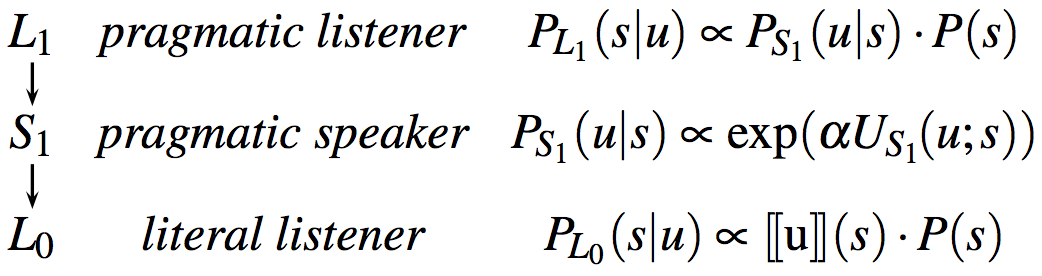
\includegraphics[width=0.5\linewidth]{vanilla-rsa.png}
	\end{center}
	\vspace{-0.3cm}
	\caption{A schematic depiction of a vanilla RSA model \parencite{problang}}
	\label{vanilla-rsa}
\end{figure*}
Putting all the elements together results in the vanilla version of an RSA-model (Fig. \ref{vanilla-rsa}).

The crucial illustration of the RSA mechanism is the difference between the distributions inferred by $L_0$ and $L_1$ upon receiving the same utterance 'blue'. The social reasoning about an utterance-generating speaker-model incorporated in $L_1$, which differentiates it from $L_0$ who acts according to literal semantics only, is crucial for the pattern of interpretation we observe: $L_1$ infers that the speaker is more likely to mean the blue square because if she had meant the blue circle, she could have said 'circle', which would have been less ambiguous, and therefore more informative - that is, $L_1$ \emph{explains away} the other potentially intended state (Table \ref{rsa-l1}). In contrast, $L_0$ infers equal probability of both the blue square and the blue circle (Table \ref{rsa-l0}). Crucially, this pattern predicted by the RSA-model is well in line with rational behaviour of humans gathered empirically in such reference game scenarios, showing that human interlocutors make use of more than just the literal semantics of their words when communicating \parencite{frank2012predicting, problang}.

Having set the basic building blocks of RSA models, some more sophisticated extensions of RSA relevant for modelling adjectives should be mentioned. 
As pointed out above, the speaker is assumed to be a rational agent producing utterances of optimal utility with respect to some specific \emph{conversational goal} determined by discourse, also called \emph{question under discussion (QUD)}  \parencite{lassiter2017adjectival}. The communication is structured so as to maximize the pobability that the listener infers the intended \emph{answer to this QUD}. In the example above, the QUD was to determine the intended referent, and the intended answer was 'blue square'.   

%note that these exist as part of L1's reasoning \parencite{lassiter2017adjectival}
\section{Previous RSA models of gradable adjectives}
In this section, previous models of gradable adjectives are discussed, showing that RSA is a flexible tool suitable to integrate pragmatic reasoning about multiple variables listeners might be uncertain about.
%threshold semantics, where the threshold is probabilistically inferred \parencite{lassiter2017adjectival} for a given comparison class.

\textcite{lassiter2013context} first provided a model of gradable adjective interpretation within the RSA-framework, showing that pragmatic reasoning can capture their meaning via inference over the latent standard of comparison variable $\theta$ underlying the vague semantics (s. Chapter \ref{chapter02}). %Importantly, probabilistic reasoning provides tools to capture uncertainty over certain aspects of the message, in this particular case - the speaker’s intended meaning of the adjectival utterance.  
The proposed model builds upon the standard RSA model with three levels, adding one crucial extension: the pragmatic listener $L_1$ jointly infers the value of the threshold $\theta$ along with the state of the world $s$ - i.e., the degree to which a referent possesses the property described by the adjective:

$$P_{L_1} (s, \theta | u) \propto P_{S_1} (u | s, \theta) \times P (s) \times P(\theta)$$ 

The model formalized the meaning of gradable adjectives in terms of degree-semantics, assuming that the lexical entry of the adjective specifies the underlying scale and its polarity (cf. chapter \ref{chapter02}):
$$\llbracket u \rrbracket_{\theta} (s) = s > \theta$$
However, the literal meaning of the adjective by itself is underspecified - it depends on the pragmatically recovered $\theta$, which in turn depends on the comparison class used in the particular context; yet, like vanilla RSA the model is anchored in the literal interpretation of the adjective applied to a referent at the level of $L_0$.  
So in order to allow specifying the $L_0$ which requires the computation of the truth-value of an utterance for a given state, the authors proposed $L_1$ consider all possible assignments of the latent variable value $\theta$, given a prior over that variable $P(\theta)$. Crucially, the state prior $P(s)$ encodes any prior knowledge about \emph{likely property degrees for a specific comparison class} which the referent's property might have in order to be felicitously described by the adjective, which $\theta$ depends on. For instance, the difference in the meanings of \emph{big} in 'big for a tree' and 'big for a pug' would be encoded different  priors over the likely properties and thresholds. It is common practice to quantify this prior knowledge empirically via prior elicitation experiments \parencite{problang}.

The assumed $\theta$ values are then iteratively passed down through the model. Given a particular value, the speaker-model can be specified:
$$P_{S_1} (u | s, \theta) \propto exp(\alpha \: log (P_{L_0} (s | u, \theta) - C(u)) )$$

Then, in contrast to $L_1$ who is uncertain about $\theta$, $L_0$ encodes the literal listener who interprets the utterance literally, so she gets $\theta$ passed down and infers the state distribution consistent with this particular $\theta$ assignment and the observed adjective $u$:
$$P_{L_0} (s | u, \theta) = P_{L_0} (s | \llbracket u \rrbracket ^\theta = 1 ) \propto \llbracket u \rrbracket ^\theta (s) \times P(s)$$

So putting all the layers together, $L_1$ can compute a joint posterior distribution over all possible combinations of states and values of the latent threshold $\theta$ lifted to the level of the pragmatic listener. Notably, \textcite{lassiter2013context} assume the relevant comparison class to be supplied to the listener, such that she is only uncertain about the standard of comparison. Yet as discussed in chapter \ref{chapter03} and shown empirically in chapter \ref{chapter04}, listeners flexibly reason about the intended comparison class, given multiple a priori plausible options in absence of an explicit \emph{for}-phrase.

\textcite{tessler2017warm} introduced an RSA-model of gradable adjectives accounting for flexible reasoning about the relevant comparison class via world knowledge. In particular, in the proposed model the listener is not only uncertain about the standard of comparison $\theta$, but also about the specificity of the relevant comparison class $c$ (is it the superordinate or subordinate category of the referent?), given prior knowledge about typical property distributions in each category; therefore, listeners were assumed to know the a priori probability that an adjective could felicitously apply to a referent assuming a specific comparison class.
Similarly to the model proposed by \textcite{lassiter2013context}, the pragmatic listener 'simulated' the utterance-generating process assuming all possible value assignments of the lifted $\theta$ variable.
Then, the pragmatic listener jointly infers the property degree $s$, the threshold $\theta$ and the relevant comparison class $c$, given a simple adjectival utterance $u$ of the form '\emph{PRON} is \emph{ADJ}' said of a referent, whose \emph{subordinate category is known to the listener}:

$$P_{L_1}(s, \theta, c | u) \propto P_{S_1} ( u | s, \theta, c) \times P(s | c_{sub}) \times P(c) \times P(\theta)$$  
That is, listeners reason about how a rational speaker $P_{S_1}$ would behave in order to communicate a specific property, given a comparison class and a threshold, together with their prior knowledge about what property degrees are plausible given the subordinate category $P(s | c _{sub})$ the referent belongs to, and their prior beliefs $P(c)$ about which comparison class categories are likely to be used and what properties are likely to be talked about ($P(\theta)$). Accordingly, the speaker-model $P_{S_1}( u | s, \theta, c)$ can be specified assuming particular values of a property, the comparison class and the threshold:

$$P_{S_1}( u | s, \theta, c) \propto exp(\alpha \: log P_{L_0} (s | u, \theta, c))$$

The $L_0$ again specifies a literal listener who interprets the adjective $u$ according to its literal semantics, assuming a particular comparison class $c$ and $\theta$:

$$P_{L_0}(s | u, \theta, c) \propto \llbracket u \rrbracket_{\theta} (s) \times P( s | c)$$  
Importantly, $L_0$ now samples states according to a prior $P(s|c)$ specified by the received comparison class $c$, thus integrating the comparison class into the literal semantics. 

Since the predictions of this model strongly depend on prior world knowledge, it is important how the property priors given different comparison classes are specified. \textcite{tessler2017warm} fixed superordinate property distributions as $\mathcal{N} (0, 1)$ and subordinate property distributions as $\mathcal{N}(\mu_{sub}, \sigma_{sub})$, inferring the paramters of subordinate distributions from experimental data. The comparison class prior $P(c)$ was approxiamted as the empirical Google WebGram frequency of usage of the respective comparison class labels.

\textcite{tessler2017warm} showed that the model captures human inferences discussed in chapter \ref{2.4.} very well, confirming the role of world knowledge for comparison class inference. 
% potential spot to integrate Dan Yurovsky's work 

However, this model only included the influence of world knowledge as a driver of comparison class inference, and the model included simple underspecified utterances of the form 'He is tall' only. In the following section, a further extension of previous RSA models allowing for flexible comparison class inference as driven by the context, the noun and its syntactic cues is proposed, incorporating the reference-predication trade-off hypothesis. 

\section{Refpred-RSA}
\pt{tbd}